% $Id: introduction.tex 34630 2013-04-29 22:53:51Z roldeman $

\section{The determination of systematic errors}
\label{sec:closureTests}

As the $\alpha_T$ analysis aims to rely as little on simulation as possible possible, systematic errors are determined via a procedure of closure tests. Various background estimation methods and assumptions made within the analysis are probed by using different regions of control samples to predict one another. The yield in an $N_{jet}$ and $H_T$ bin of region A, $N_{obs}^A$, is used to predict region B, $N_{pred}^B$, with:
\begin{equation}
  N_{pred}^B(H_T,N_{jet}) = \frac{N_{\rm MC}^
      B(H_T,N_{jet})}{N_{\rm MC}^A(H_T,N_{jet})} \times 
      N_{obs}^{\rm A}(H_T,N_{jet})   
\end{equation}
where we use the ratio of yields in MC simulation to calculate the appropriate transfer factors. For a variety of tests, the ratio $\frac{N_{obs}-N_{pred}}{N_{pred}}$ is calculated. In each bin the systematic is determined with the variance, $\sigma^2$ and the weighted mean of the points: 
\begin{equation}
\textrm{syst.} = \sqrt{\sigma^2+\textrm{mean}^2}.
\end{equation}
In the case of perfect closure, the mean and variance will be zero. However, due to the statistical limitations of the control samples, we can only determine the systematics to within a certain accuracy. Provided a suitable set of tests has been chosen, any bias in the data will always be covered by the systematic calculation with this method.
\\\\
Despite the fact that we do not have any $13$~TeV data, it is possible to investigate the degree of statistical power available to determine the systematics with MC. Despite the fact that using MC to predict itself will close by completion, the variance term contributes to the systematic. For a set of tests chosen to probe the background prediction methods we are intending to use, the closure tests in simulation can be seen in Fig.~\ref{fig:closureTests}.
\\\\
With the introduction of $\cancel{H_T}$ event categorisation, ongoing development of the closure tests is ongoing to understand the effect of this variable on the systematic error calculation.

\begin{figure}[h!]
  \centering
  \subfigure[Legend showing which sub sample of a closure test is used to predict which other sub sample]{
    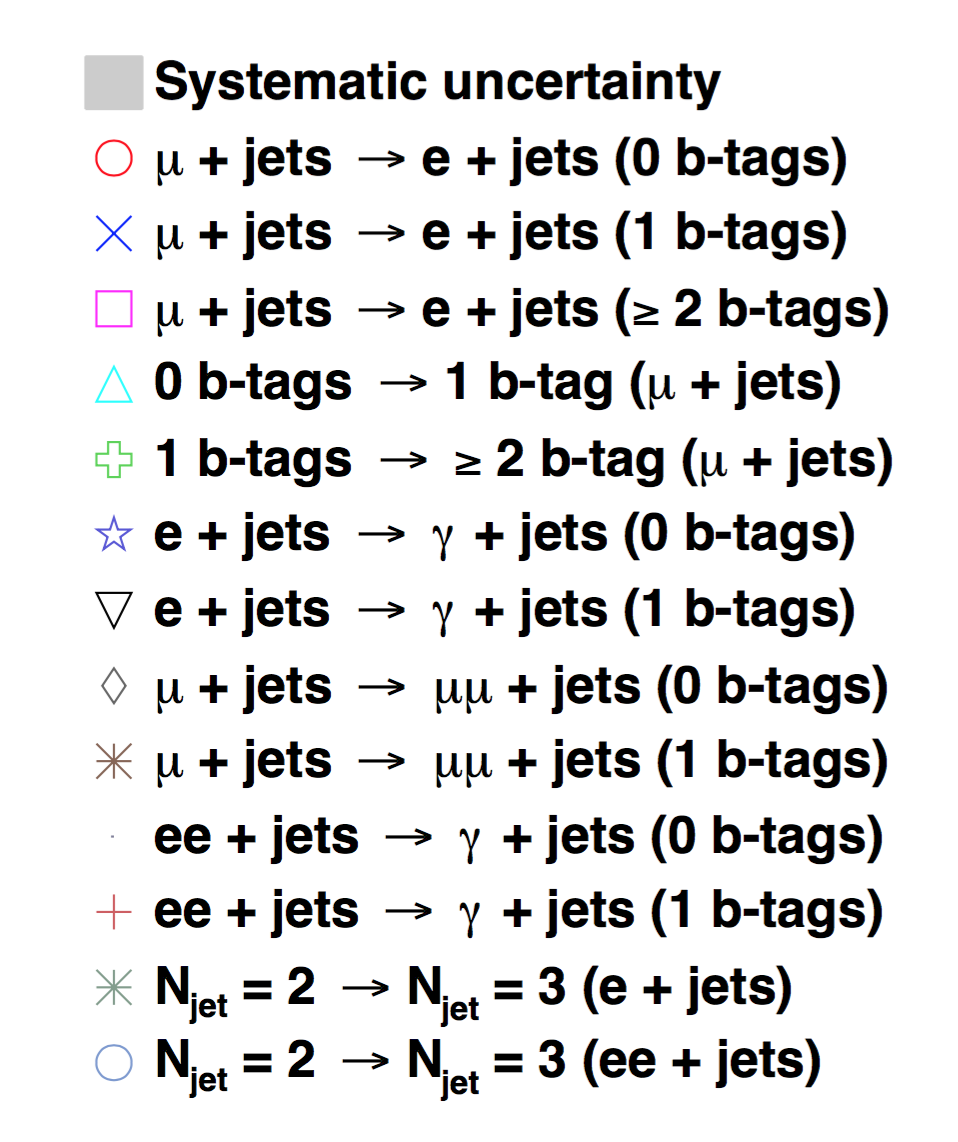
\includegraphics[width=0.3\textwidth]{closureLegend}
  }~~
  \subfigure[Closure tests in the $N_{jet}=2$ bins]{
    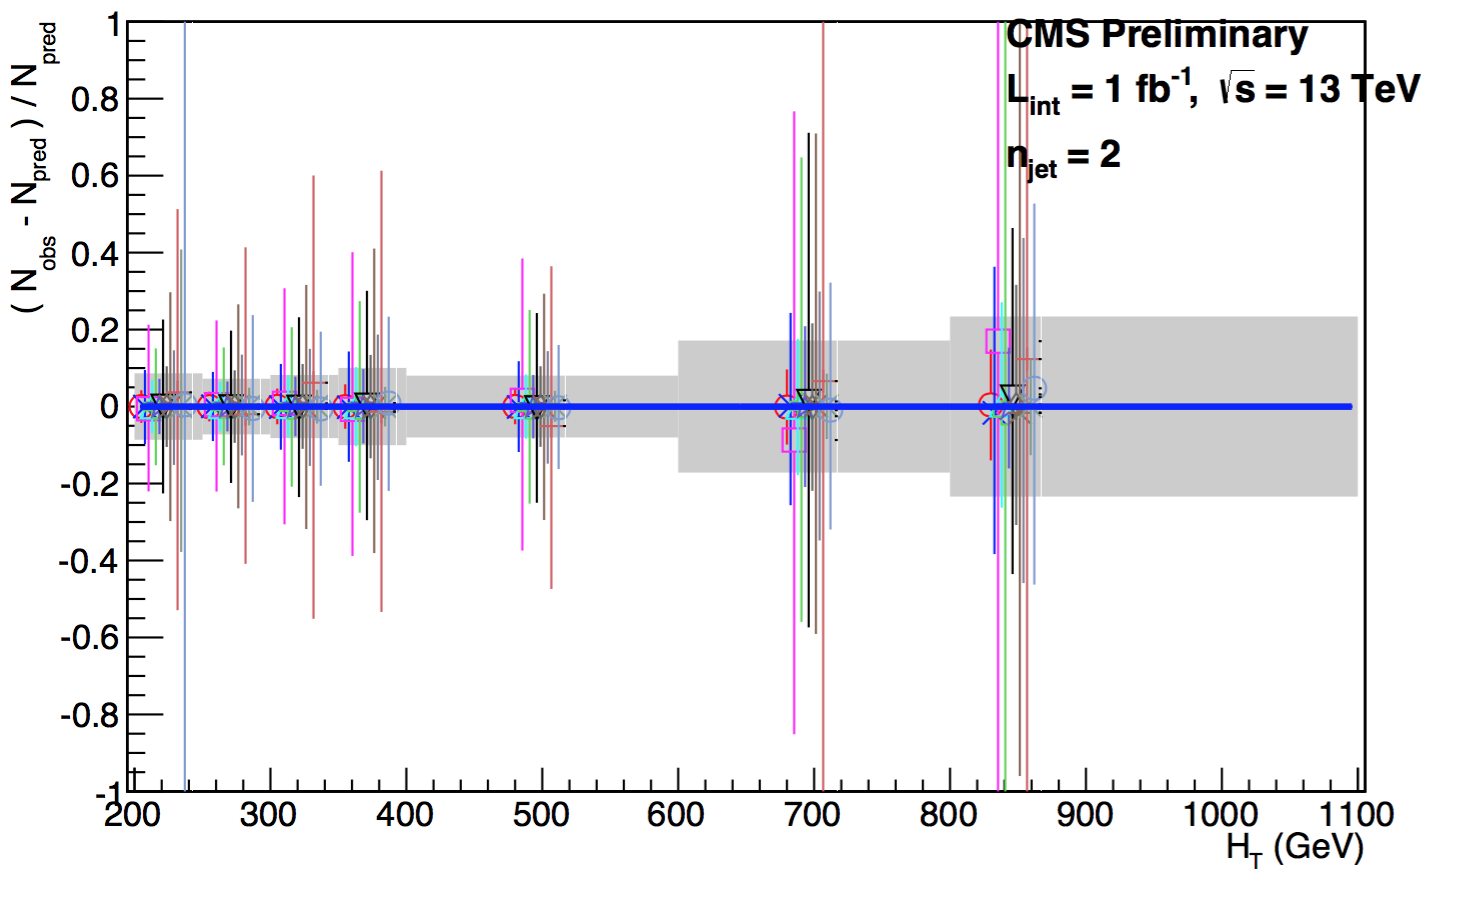
\includegraphics[width=0.7\textwidth]{closureTesteq2j}
  }
  \\
  \caption{\label{fig:closureTests} Closure tests using $13$~TeV MC simulation. As MC is used to predict itself they close by construction, but allow for the determination of the statistical power of the control samples used by the analysis.}
\end{figure}